\documentclass[a4paper,kulak]{kulakarticle} %options: kul or kulak (default)

\usepackage[utf8]{inputenc}
\usepackage[dutch]{babel}
\usepackage{wrapfig}
\usepackage{graphicx}
\usepackage{subcaption}
\usepackage{float}

\date{Academiejaar 2018 -- 2019}
\address{
  Informatica \\
  Statistische modellen en data-analyse \\
  Prof. Van Aelst, Stijn Rebry}
\title{Opdracht 2}
\author{Thomas Bamelis, Michiel Jonckheere}


\begin{document}

\maketitle

\section*{Inleiding}
In dit verslag analyseren we de gegevens van airbnb gemeten in 2019 van de steden Antwerpen, Brussel en Gent. 
De data bevat in totaal ongeveer 11.000 samples.
We analyseren de prijs in functie van het type, de stad en de buurt van het bedrijf.
Daarna proberen we een regressiemodel op te stellen voor de huurprijs en dit model te evalueren en te interpreteren.
Als laatste passen we logistische regressie toe om te voorspellen of een verblijf al dan niet wordt vast verhuurd in plaats van enkel voor korte periodes.\\
\textit{Opmerking:} als in dit verslag een p-waarde als nagenoeg 0 wordt beschreven, betekent dit dat de p-waarde voor underflow zorgde in het computersysteem (< 2.2e-16).
Indien het significantieniveau niet vermeld staat wordt 0.05 gehanteerd.

\section{Ligging en type verblijf}
In deze sectie analyseren we de prijs in functie van het type, de stad en de buurt van het bedrijf.
We analyseren of de stad nog significant is als de buurt wordt inbegrepen en de buurt als het type verblijd wordt meegerekend.
Deze laatste omdat in bepaalde buurten misschien hoofdzakelijk een bepaald soort type verblijf aanwezig is.
\subsection{type verblijf vs huurprijs} \label{sec:pt}
\begin{wrapfigure}{r}{0.5\textwidth}
	\begin{center}
		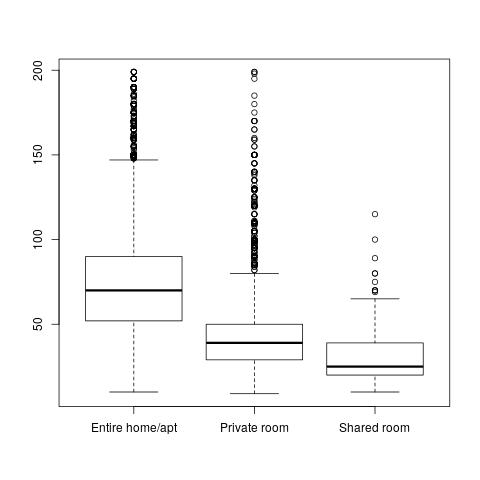
\includegraphics[width=0.35\textwidth]{boxplotPrijsCity.jpg}
	\end{center}
	\caption{Boxplot type vs prijs.}
	\label{fig:bpc}
\end{wrapfigure}
Een boxplot van de prijs tegenover de stad (\ref{fig:bpc}) zonder de outliers lijkt te suggereren  dat er wel degelijk een verschil blijkt te zijn tussen de types van de verblijven, en dan vooral tussen een volledig huis/appartement en de rest.
Om overzicht te behouden hebben we de bovenste outliers uit de figuur gelaten, waarvan er nog 705 tussen 150 en 1500 lagen en nog 8 hoger dan 1500 met een maximum van 8944. 
We analyseren eerst de verdeling van de prijs om beter over het komend werk te kunnen redeneren.
De prijs lijkt aan de hand van figuur \ref{fig:pv} een redelijke klokcurve voor te stellen met echter een zeer lichte linkerstaart en een heel erg zware rechterstaart. 
Opnieuw werden de grote outliers niet in de figuur opgenomen.
Een normale kwantielplot van de prijs lijkt totaal niet normaal verdeeld door de enorm zware outliers en de knik in de curve. 
Een schatting van de lambda voor een Box-Cox transformatie raad -0.2549 aan als lambda, waardoor we een transformatie van -1/4 toepassen op de prijs.
Het resultaat is te zien in figuur \ref{fig:qqbp}, wat een zeer duidelijke verbetering toont op het vlak van normaliteit.
Deze transformatie gaf de beste verbetering van alle geteste transformaties (log, sqrt, loglog).
\begin{figure}[H]
	\centering
	\begin{subfigure}[b]{0.45\textwidth}
		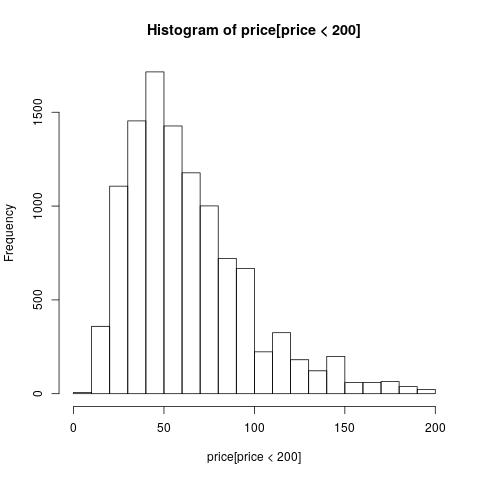
\includegraphics[width=\textwidth]{prijsVis.jpg}
		\caption{Visualisatie van de prijs.}
		\label{fig:pv}
	\end{subfigure}
	~ %add desired spacing between images, e. g. ~, \quad, \qquad, \hfill etc. 
	%(or a blank line to force the subfigure onto a new line)
	\begin{subfigure}[b]{0.45\textwidth}
		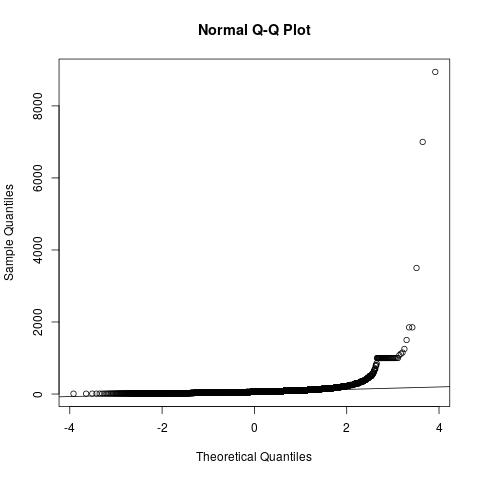
\includegraphics[width=\textwidth]{qqp.jpg}
		\caption{Kwantielplot prijs}
		\label{fig:qqp}
	\end{subfigure}
	~
	\begin{subfigure}[b]{0.45\textwidth}
		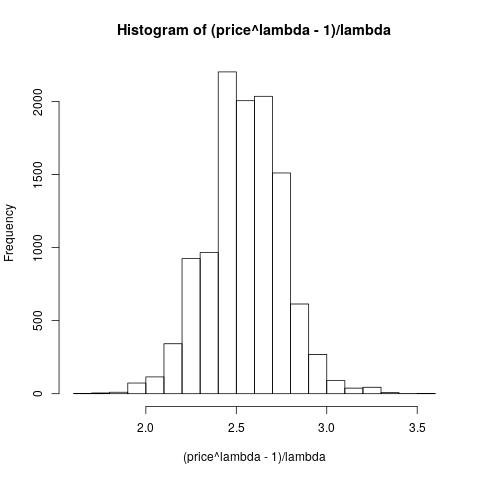
\includegraphics[width=\textwidth]{prijsB.jpg}
		\caption{Visualisatie Box-Cox -1/4 prijs}
		\label{fig:bpv}
	\end{subfigure}
	~ %add desired spacing between images, e. g. ~, \quad, \qquad, \hfill etc. 
	%(or a blank line to force the subfigure onto a new line)
	\begin{subfigure}[b]{0.45\textwidth}
		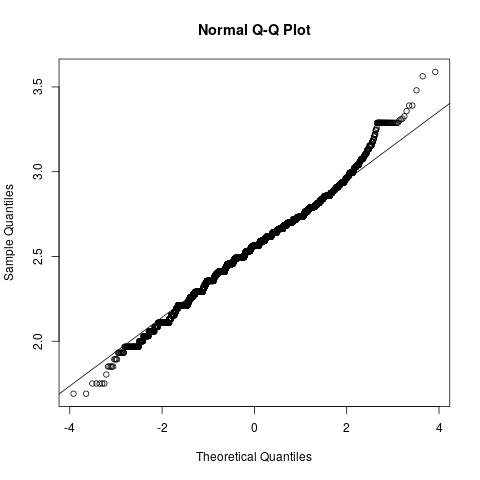
\includegraphics[width=\textwidth]{qqbp.jpg}
		\caption{Kwantielplot Box-Cox -1/4 prijs}
		\label{fig:qqbp}
	\end{subfigure}
\end{figure}


Na de residuals bekeken te hebben van de modellen waarbij transformaties van de prijs voorspeld worden aan de hand van het type, vonden we dat de Box-Cox transformatie er als beste transformatie uitkwam (figuur \ref{fig:pcqq}).
De Levene test toont aan dat er heteroscedasticiteit is van de varianties tussen de verschillende groepen met een p-waarde van nagenoeg 0, wat aannemelijk lijkt gegeven figuur \ref{fig:bpc}.
Een kwantielplot van de gestandardiseerde residuals toont ook te zware staarten (\ref{fig:pcqq}), waardoor we concluderen dat ze niet normaal verdeeld zijn.
Het aantal samples is te groot om een Shapiro test op uit te voeren.
Een plot van de residuals tegenover de index (figuur \ref{fig:pcisr}) toont geen afhankelijkheid ``in de tijd''.
Door de heteroscedasticiteit en het niet normaal zijn van de residuals zijn de modelveronderstellingen voor de relevante testen niet voldaan, onze bevindingen moeten daarom met een korrel zout genomen worden.\\
Het model verwierp de f-test (p-waarde nagenoeg 0) en t-test voor alle variabelen (p-waarde nagenoeg 0 voor alle categorieën). 
De R-squared en adjusted R-squared  waren echter maar 0.268.
De weighted least square methode toonde geen verbeteringen op het model na 1 iteratie. 
De anova methode toont alsook aan dat het type verblijf effectief significant is voor de prijs met een p-waarde van nagenoeg nul.
De tukey-test toont verder aan dat de verschillende soorten kamers onderling ook genoeg verschillen van elkaar (alle combinaties nagenoeg 0). \\
Conclusie: het type verblijf is significant voor de prijs en de types verschillen onderling allemaal in prijs. Volgens de coëfficiënten van het model is de prijs als volgt gerangschikt: 
volledig huis app. > privé kamer > gedeelde kamer.
Deze bevindingen stroken met de vermoedens van de realiteit.

\begin{figure}[H]
	\centering
	\begin{subfigure}[b]{0.45\textwidth}
		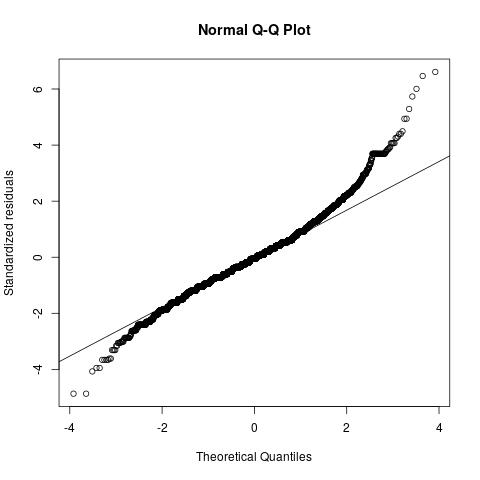
\includegraphics[width=\textwidth]{pcqq.jpeg}
		\caption{Kwantielplot gestandardiseerde residuals}
		\label{fig:pcqq}
	\end{subfigure}
	~ %add desired spacing between images, e. g. ~, \quad, \qquad, \hfill etc. 
	%(or a blank line to force the subfigure onto a new line)
	\begin{subfigure}[b]{0.45\textwidth}
		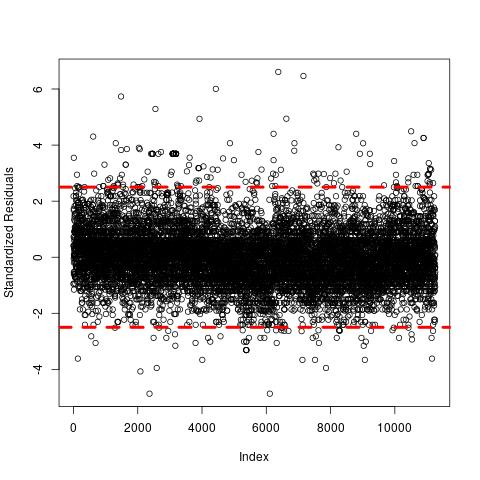
\includegraphics[width=\textwidth]{pcisr.jpeg}
		\caption{Index vs gest. residuals}
		\label{fig:pcisr}
	\end{subfigure}
\end{figure}

\subsection{stad vs huurprijs}
De boxplot zonder outliers (figuur \ref{fig:bpcit}) suggereert  dat er niet veel verschil is in de gemiddelde prijs per stad. Antwerpen en Gent zijn nagenoeg het zelfde, enkel de prijzen in Brussel liggen wat lager. \\
We nemen opnieuw dezelfde transformatie op de prijs zoals in sectie \ref{sec:pt}.
We zien dat de residuals niet normaal verdeeld zijn (figuur \ref{fig:qqboxcit}), waardoor onze bevindingen opnieuw niet steenhard mogen genomen worden. De Levene test kan echter niet verwerpen dat er homoscedasticiteit is op significantieniveau 0.05 met een p-waarde van 0.1454, waardoor de testen toch al serieuzer mogen worden genomen dan in sectie \ref{sec:pt}\\
Het model verwerpt de f-test (p-waarde nagenoeg 0) en t-test voor de variabelen van Antwerpen (= het intercept) en Brussel (p-waarde nagenoeg 0), maar Gent is niet verworpen op significantieniveau 0.05 met een p-waarde van 0.068. 
Er moet rekening meegehouden worden dat Antwerpen ``voorang'' krijgt aangezien het het intercept is, en de gelijkenissen tussen Antwerpen en Gent uit figuur \ref*{fig:bpcit} dit kunnen verklaren. 
De reden dat Gent dus niet verworpen is, is omdat hij heel sterk op Antwerpen lijkt, wat dus betekent dat beiden niet significant verschillen qua prijs.
En het dus niet perse Gent die slechter is dan de andere twee. Het kleine verschil in de coëfficiënten bevestigd dat.
Aov zegt dat de stad significant is voor de prijs op significantieniveau 0.05 met een p-waarde van nagenoeg 0. 
De residuals zijn niet afhankelijk van de tijd/index, dit volgt uit figuur \ref{fig:indc}.
De R-squared van dit model is 0.0226 en de adjusted is 0.0224, wat dus opnieuw niet goed is.
De Tukey-test verwerpt sterk dat er geen verschil zou zijn tussen Brussel en de andere twee steden. Maar Gent en Antwerpen worden niet verworpen op significantieniveau 0.05 met een p-waarde van 0.162, wat opnieuw onze vermoedens bevestigd. 
Het effect van Brussel is ook veel sterker dan die van Antwerpen en Gent. 
Conclusie: de stad is significant voor de prijs. Er is een prijsverschil tussen Brussel en de andere 2 steden, maar er is geen significant prijsverschil tussen Antwerpen en Gent.
De coëfficiënten van het model vertellen dat Brussel goedkoper is dan de andere 2 steden, wat strookt met de boxplot op figuur \ref{fig:bpcit}.

\begin{figure}[H]
	\centering
	\begin{subfigure}[b]{0.3\textwidth}
		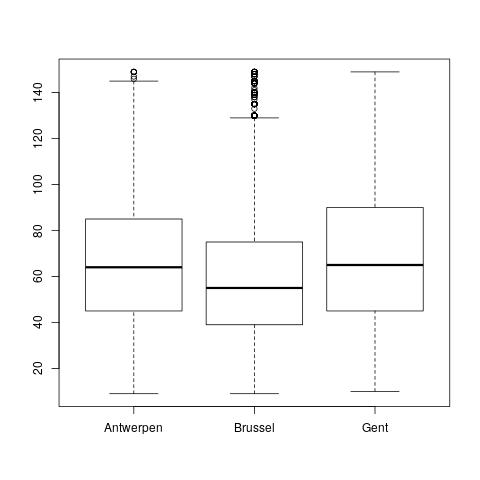
\includegraphics[width=\textwidth]{boxprijscity.jpg}
		\caption{Boxplot stad vs prijs.}
		\label{fig:bpcit}
	\end{subfigure}
	~ %add desired spacing between images, e. g. ~, \quad, \qquad, \hfill etc. 
	%(or a blank line to force the subfigure onto a new line)
	\begin{subfigure}[b]{0.3\textwidth}
		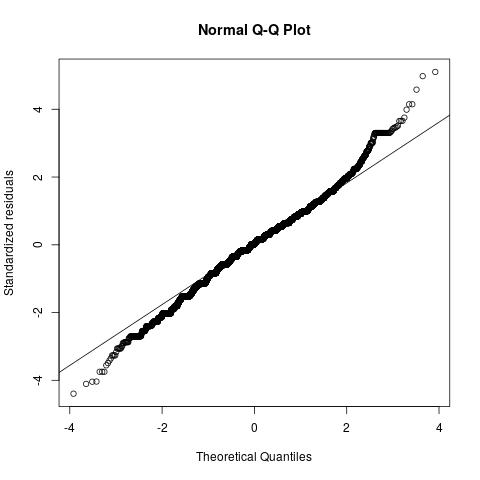
\includegraphics[width=\textwidth]{qqboxcit.jpg}
		\caption{QQplot gestandaardiseerde residuals model}
		\label{fig:qqboxcit}
	\end{subfigure}
	~
	\begin{subfigure}[b]{0.3\textwidth}
		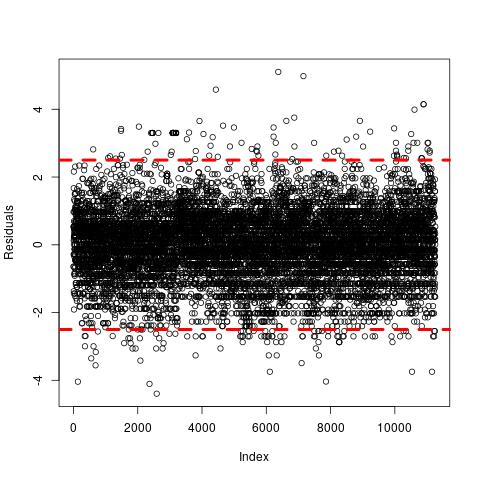
\includegraphics[width=\textwidth]{indc.jpg}
		\caption{Index vs residuals}
		\label{fig:indc}
	\end{subfigure}
\end{figure}

\subsection{Buurten}
We nemen opnieuw dezelfde transformatie op de prijs zoals in sectie \ref{sec:pt}.
Op het eerste zicht (figuur \ref{fig:boxne}) lijken de buurten niet zo veel te verschillen.
Het model waarbij we enkel neighbourhood meenemen, verwerpt de f-test met p-waarde nagenoeg 0, maar een groot deel van de neighbourhoods worden niet verworpen door de t-test op significantieniveau 0.05 (43/96). 
Door de heteroscedasticiteit doe blijkt uit een Levene test en het niet normaal zijn van de residuals (figuur \ref{fig:qqne}) zijn de modelveronderstellingen voor de relevante testen niet voldaan, onze bevindingen moeten daarom met een korrel zout genomen worden.
Residual zijn niet afhankelijk van de tijd/index (figuur \ref{fig:stdne})
Aov toont aan dat de buurt significant is met p-waarde nagenoeg 0.
De TukeyTest kan 47,6\% niet verwerpen, dus 47,6\% van de combinaties van buurten verschillen niet significant.
De R-squared is 0.099 en adjusted 0.091, wat opnieuw aan de lage kant is.
Alleen lijkt dus dat de buurt significant is in het algemeen, maar zeer veel buurten onderling te weinig verschillen.
Dit doet suggereren dat de opdeling per buurt te verfijnt is.


\begin{figure}[H]
	\centering
	\begin{subfigure}[b]{0.3\textwidth}
		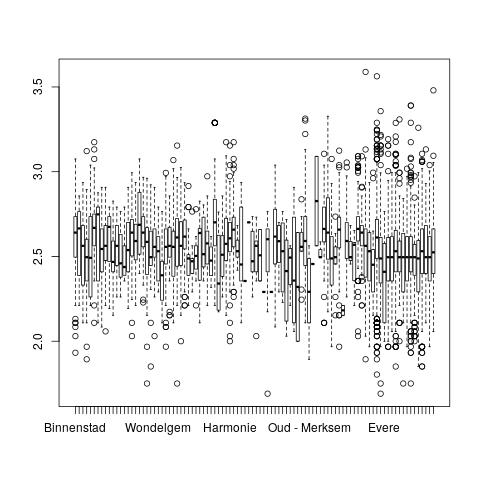
\includegraphics[width=\textwidth]{boxne.jpg}
		\caption{Boxplot buurt vs prijs.}
		\label{fig:boxne}
	\end{subfigure}
	~ %add desired spacing between images, e. g. ~, \quad, \qquad, \hfill etc. 
	%(or a blank line to force the subfigure onto a new line)
	\begin{subfigure}[b]{0.3\textwidth}
		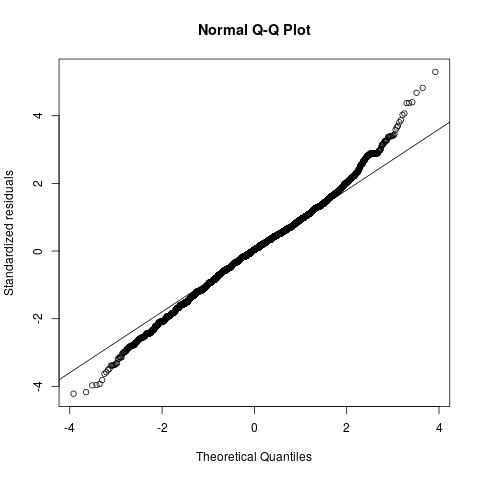
\includegraphics[width=\textwidth]{qqne.jpg}
		\caption{QQplot gestandaardiseerde residuals model}
		\label{fig:qqne}
	\end{subfigure}
	~
	\begin{subfigure}[b]{0.3\textwidth}
		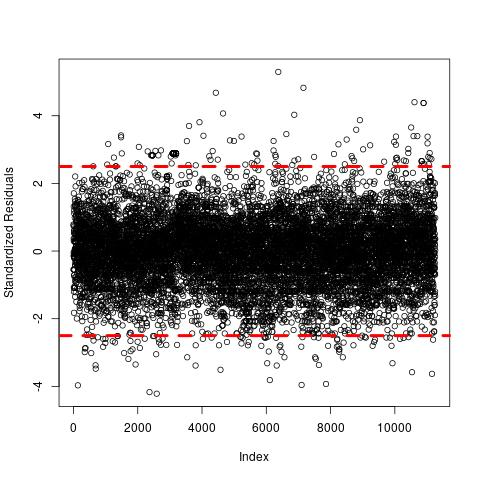
\includegraphics[width=\textwidth]{stdne.jpg}
		\caption{Index vs residuals}
		\label{fig:stdne}
	\end{subfigure}
\end{figure}

\subsection{Buurten en stad}
We nemen opnieuw dezelfde transformatie op de prijs zoals in sectie \ref{sec:pt}.
Het model met de buurt en de stad verwerpt de f-test ook met p-waarde nagenoeg 0, maar een nog groter deel van  wordt niet verworpen door de t-test (54). Meer bepaald is de pwaarde van Gent zeer hoog (0.9) terwijl Antwerpen (nagenoeg 0) en Brussel (0.016, wel hoger dus) nog steeds verworpen worden (Antwerpen omdat die het intercept is). 
De R-squared is 0.099 en adjusted 0.091 en blijven dus onveranderd bij het toevoegen van de stad. Dit doet vermoeden dat beide dus sterk verbonden zijn aangezien hun gecombineerd model even slecht is als hun afzonderlijke.
Aov verwerpt echter voor beide variabelen en zegt dus dat ze beiden nog significant zijn.
De Tukey test kan nu nog 44,6\% van de combinaties verwerpen.
Deze bevindingen suggereren dat door de buurt en de stad beiden op te nemen, de significantie van Gent vs. Antwerpen miniem wordt. De Aov verwerpt niet dat een van de twee overbodig wordt, maar aangezien zeer veel variabelen de t-test falen, er geen verbetering is in de R-squared en het nog steeds hoge percentage van het niet verwerpen van de Tukey test tonen dat het origineel probleem van het te verfijnd zijn van de buurtenverdeling enkel nog maar versterkt wordt door de stad erbij te nemen.



\begin{figure}[H]
	\centering
	\begin{subfigure}[b]{0.3\textwidth}
		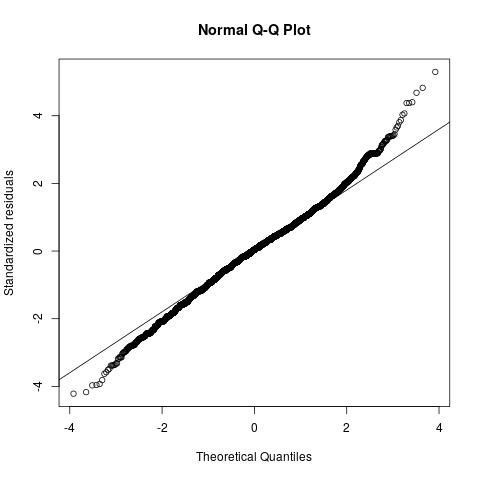
\includegraphics[width=\textwidth]{qqnes.jpg}
		\caption{QQplot gestandaardiseerde residuals model}
		\label{fig:qqnes}
	\end{subfigure}
	~
	\begin{subfigure}[b]{0.3\textwidth}
		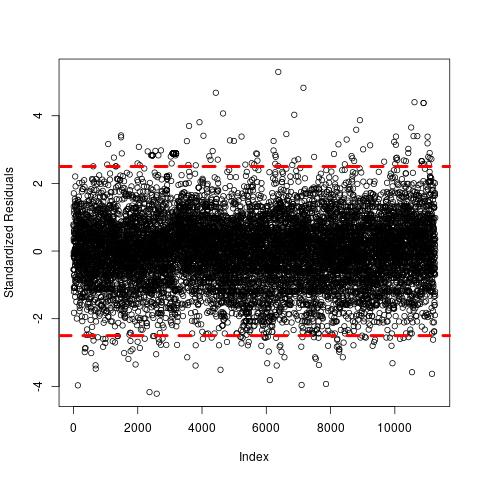
\includegraphics[width=\textwidth]{stdnes.jpg}
		\caption{Index vs residuals}
		\label{fig:stdnes}
	\end{subfigure}
\end{figure}
\begin{wrapfigure}{r}{0.4\textwidth}
	\begin{center}
		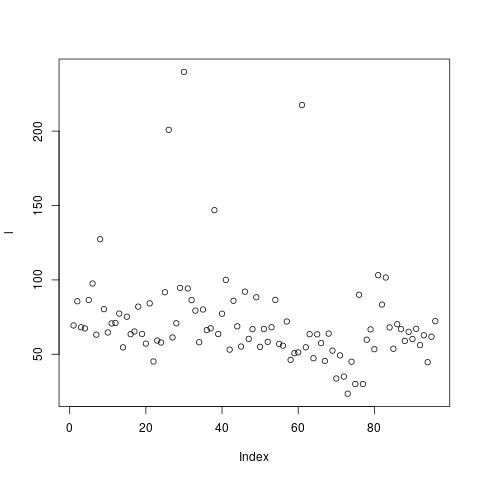
\includegraphics[width=0.35\textwidth]{pn.jpg}
	\end{center}
	\caption{Gemiddelde prijs per buurt.}
	\label{fig:pn}
\end{wrapfigure}
Figuur \ref{fig:pn} toont dat er een ongeveer 5 buurten zijn die een opvallend hogere prijs hebben dan de rest.
De gemiddelde huurprijs is 72,2 euro.
Woluwe-Saint-Pierre steekt hier sterk boven met een gemiddelde huurprijs van 240 euro.
Daarna volgt Sint Denijs Westrem met 217,5 en Oud-Berchem met 201.
Deze drie zijn significant hoger dan de rest in liggen in Brussel, Gent en Antwerpen. Niet in een bepaalde stad dus.
Dan zijn er nog 2 minder extreem prijzige gemeenten, namelijk Eilandje met 147 en Polder met 127 (beiden liggen in Antwerpen). De eerste opeenvolgende is nog maar 103.
Daarnaast zijn er nog 5 Antwerpse buurten waar de prijs ietwat lager ligt dan de rest met prijzen tussen 23,5 en 35 euro.
Deze zijn echter minder een stuk minder ver verwijdert van het gemiddelde in vergelijking met de extreem prijzige outliers.

\subsection{Buurten en type verblijf}
Op analoge manier zijn we te werk gegaan om een model op te stellen van de buurten en het type.
Opnieuw werd de f-test verworpen en 42 t-testen gefaald.
Aov verwerpt echter voor beide variabelen en acht ze dus beide significant.
Wat echter wel opmerkelijk is, is dat de R-squared sterk gestegen is van 0.099 naar 0.3281 en de adjusted van 0.091 naar 0.3222.
De R-squared van room-type alleen was ook 0.2678 en de adjusted 0.2677. De combinatie van de 2 variabelen versterk elkaar dus.
De buurt en het type verblijf maken elkaar dus niet overbodig.




\section{Model voor de huurprijs}
% todo kleine inleiding vd opdracht
commentaar thomas:\\
variabelen selectie: teveel variabelen laten vallen in het begin, nu deze variabelen gebruiken: roomtype, price, minimumnights, nbreviews, lastreviez, reviewpermonth, calchost, city, availability \\
transformaties\\
interactietermen\\

model evalueren:\\
checken op multicolineariteit checken\\
waar liggen de outliers\\
inferenties\\
5plots (pg216, residualplots)

\section{Beschikbaarheid van een verblijf}
% todo kleine inleiding vd opdracht


\section*{Besluit}

Afsluitende tekst.

\end{document}
